\chapter{Gráficas}

MATLAB dispone de una gran variedad de funciones y herramientas que
permiten crear gráficas de casi cualquier tipo, tanto en dos dimensiones
como superficies y curvas tridimensionales. Además, MATLAB proporciona
una facilidad extraordinaria para personalizar las gráficas mediante la
inclusión de anotaciones, etiquetas, mapas de colores y muchos otros
elementos que permiten una mayor legibilidad e interactividad con la
información presentada en los gráficos. En este capítulo se tratarán las
gráficas en dos dimensiones y en el espacio tridimensional.

\section{Una introducción: la función \texttt{plot}}

trazar curvas bidimensionales utilizando vectores como argumentos. Por
ejemplo si necesita graficar la función seno en el intervalo de
$-\pi$ a $\pi$, necesita definir primeramente un
vector con un determinado número de elementos para construir el dominio
a graficar y enseguida aplicar a ese vector la función matemática que
corresponda. A continuación se especifican las líneas de código
necesario para crear la gráfica antes mencionada y el resultado de
salida:

\begin{matlab}
x=-pi:pi/180:pi;
y=sin(x);
plot(x,y);
\end{matlab}


\begin{figure}[htbp]
    \centering
    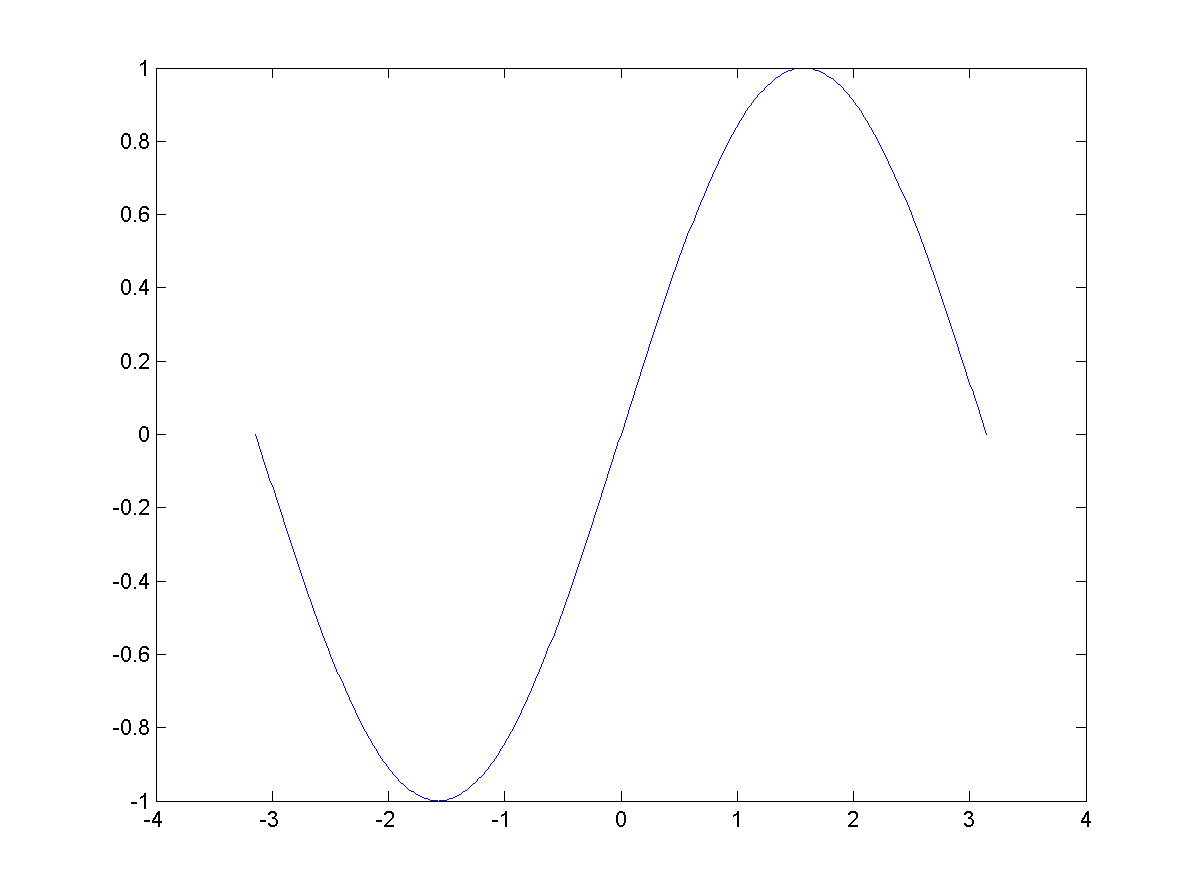
\includegraphics[width=0.65\textwidth]{images/ch4/img_4_1.png}
    \caption{Graficando una función}
    \label{fig:img_4_1}
\end{figure}


\subsection{Graficar más de una función}

Si necesita incluir dos o más gráficas en una misma ventana puede
utilizar el comando \texttt{hold\ on} para permitir que MATLAB
simplemente agregue las gráficas sin borrar las ya existentes, por
ejemplo:

\begin{matlab}
x=-pi:pi/180:pi;
y1=sin(x);
y2=cos(x);
y3=cos(x+pi/3);
hold on
plot(x,y1);
plot(x,y2);
plot(x,y3);
\end{matlab}

\begin{figure}[htbp]
    \centering
    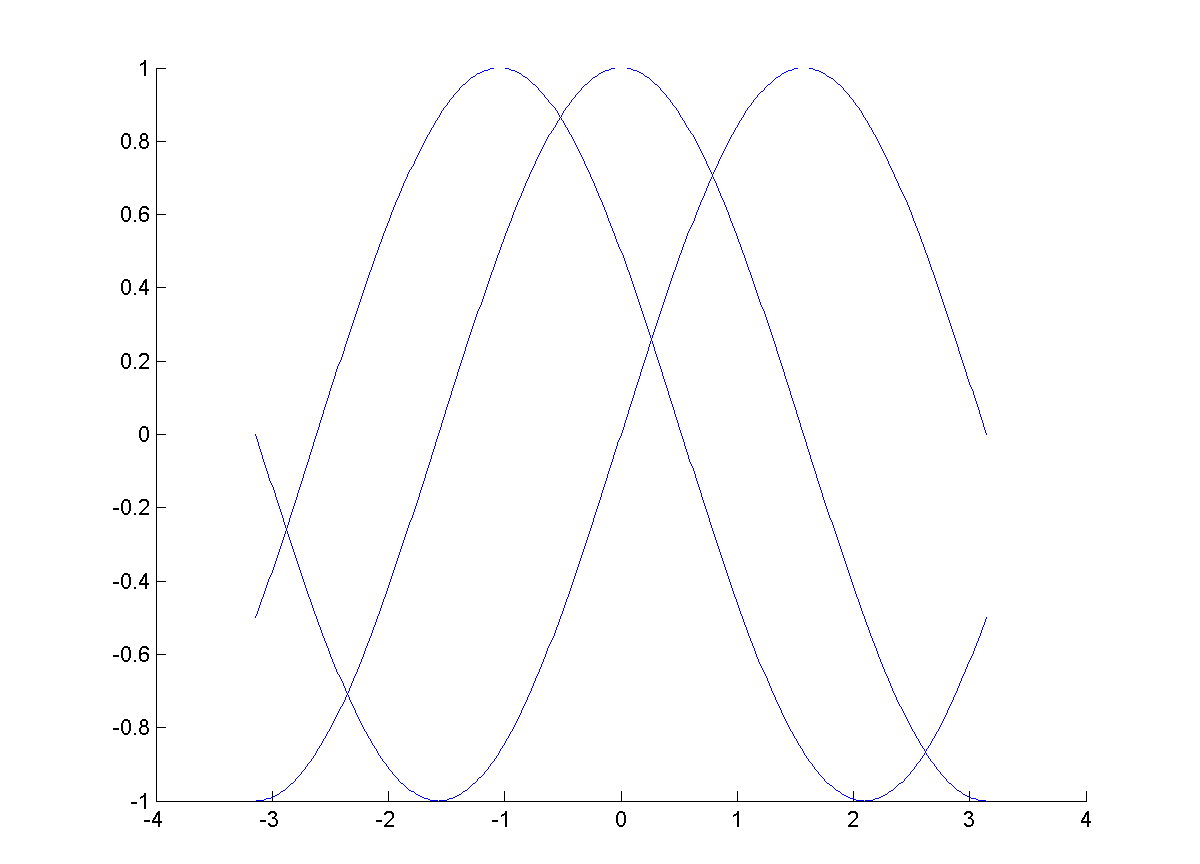
\includegraphics[width=0.65\textwidth]{images/ch4/img_4_2.png}
    \caption{Varias gráficas utilizando \texttt{hold on}}
    \label{fig:img_4_2}
\end{figure}

Lo anterior funciona incluso para cuando se tienen intervalos
diferentes. Si necesita graficar dos o más funciones en un mismo
intervalo, es decir utilizando el mismo vector como variable
independiente, puede utilizar la siguiente forma más compacta para
agregar más de una función sin recurrir al comando descrito con
anterioridad:

\begin{matlab}
x=-pi:pi/180:pi;
y1=sin(x);
y2=cos(x);
y3=cos(x+pi/3);
plot(x,[y1;y2;y3]);
\end{matlab}

\begin{figure}[htbp]
    \centering
    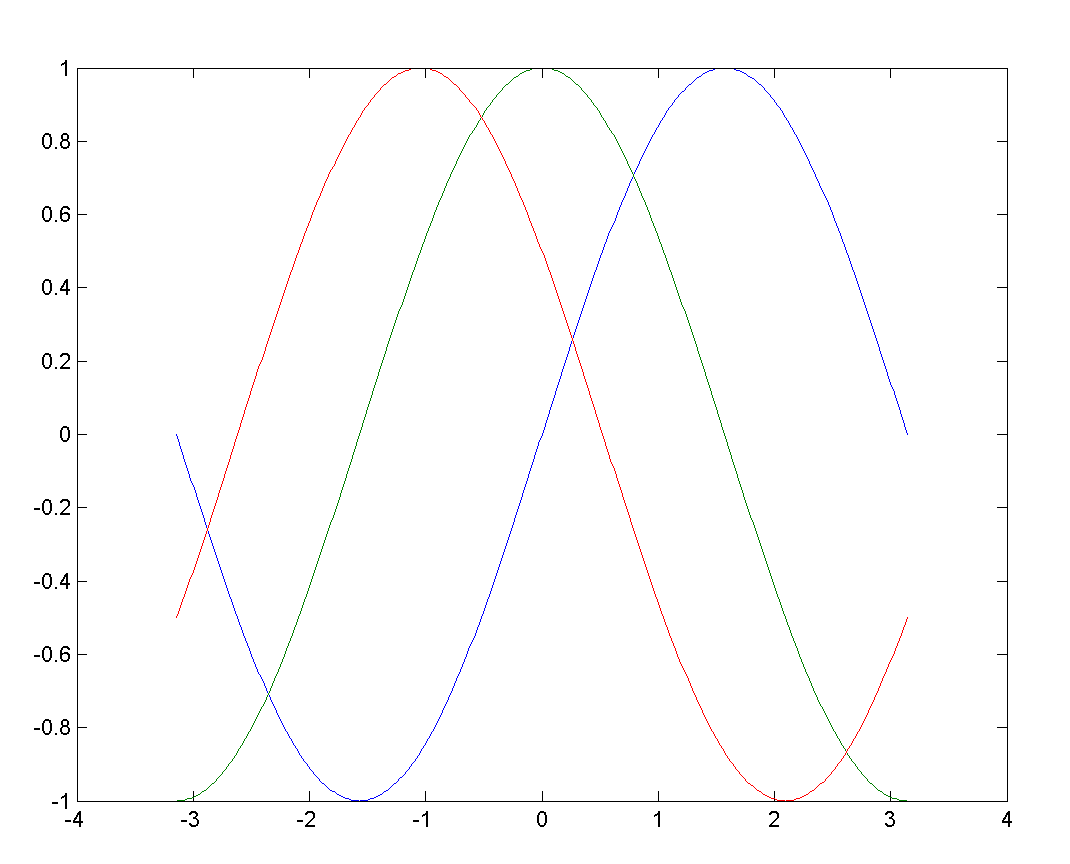
\includegraphics[width=0.65\textwidth]{images/ch4/img_4_3.png}
    \caption{Varias gráficas usando concatenación vectorial}
    \label{fig:img_4_3}
\end{figure}

En lugar de utilizar \texttt{hold on} puede configurar la propiedad
\texttt{NextPlot} del axes de tal manera que las gráficas sean agregadas
sin borrar los objetos que pertenecen al axes. Lo anterior se logra con
la siguiente línea de código:

\begin{matlab}
set(gca, 'NextPlot', 'add');
\end{matlab}

Quizá lo anterior resulte un poco avanzado para comenzar, pero puede
tomarse simplemente como una observación muy útil de que en MATLAB
pueden implementarse diversas soluciones a un mismo problema o
requerimiento.

\section{Configurar propiedades de las gráficas}

\subsection{Añadir etiquetas, leyendas y títulos}

En la sección anterior se han visto los pasos para mínimos para trazar
una gráfica, pero ésta todavía puede resultar poco útil dado que no
contiene información de ningún tipo acerca de los datos graficados. Es
posible añadir etiquetas a los ejes con las funciones xlabel, ylabel y
zlabel, además de poder añadir una identificación de una determinada
curva mediante la función \texttt{legend} e incluso colocar un título en
la parte superior con la función \texttt{title}:

\begin{matlab}
x=-pi:pi/180:pi;
y=sin(x);
plot(x,y);
xlabel('Eje X');
ylabel('Eje Y');
title('Gráfica función seno');
legend('f(x)=sin(x)');
\end{matlab}

\begin{figure}[htbp]
    \centering
    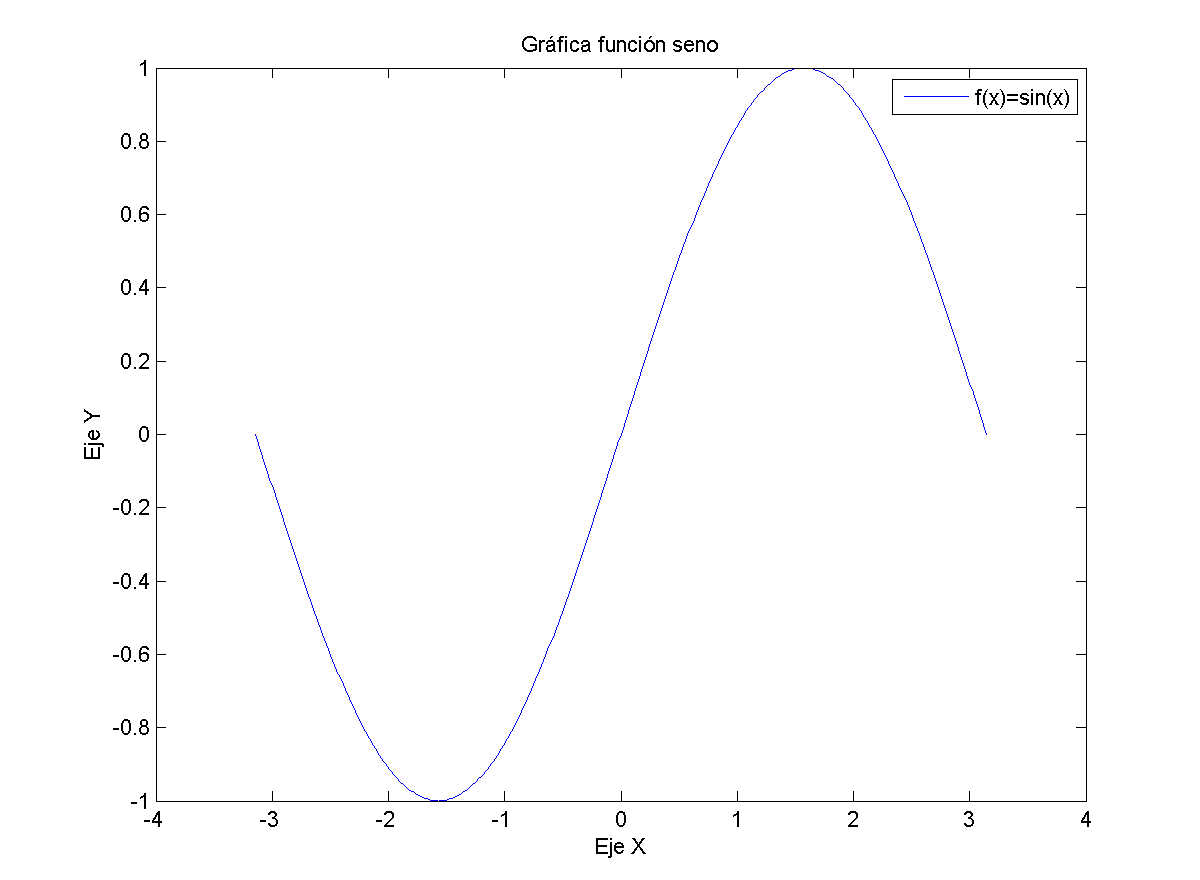
\includegraphics[width=0.65\textwidth]{images/ch4/img_4_4.png}
    \caption{Gráfica con etiquetas y leyenda}
    \label{fig:img_4_4}
\end{figure}

Las gráficas anteriores se han trazado utilizando el estilo por defecto
que emplea MATLAB, es decir, una línea continua en color azul, pero es
posible modificar el color, grosor y el estilo de línea de las gráficas
de modo que se ajuste a los requerimientos o a las exigencias visuales
de cada individuo.

\subsection{Modificando el color de línea}

Para modificar el color de una gráfica basta con añadir como tercer
argumento de la función plot uno de los modificadores de color que se
indican en la siguiente tabla:


\begin{table}[h!]
\centering
% \rowcolors{1}{}{gray!20}
\begin{tabular}{p{3cm} >{\tt}P{3cm}}
\hline
\Centering\bfseries Color  & \normalfont\bfseries Modificador \\
\hline 
Rojo  &  r \\
verde &  g \\
Azul  &  b \\
Cyan  &  c \\
Magenta &  m \\
Amarillo & y \\
Negro  & k \\
Blanco & w \\
\hline
\end{tabular}
\caption{Conversiones entre tipos numéricos}
\end{table}



La sintaxis de la función plot para una línea color verde sería:

\begin{matlab}
plot(x,y,'g');
\end{matlab}

Además de los modificadores anteriores puede utilizarse un vector de
tres elementos RGB para especificar el color, pero en este caso tiene
que especificarse como argumento la propiedad que se modifica, es decir
color, con lo cual la sintaxis bajo este método para trazar una línea
color verde sería como sigue:

\begin{matlab}
plot(x,y,'color',[0 1 0]);
\end{matlab}

\subsection{Configurar ejes (función axis)}

El comando / función axis permite hacer modificaciones a la apariencia y
escala de los ejes en los cuales se trazan las gráficas. La sintaxis
varía dependiendo de la característica a modificar.

\subsubsection{Estableciendo los límites de una gráfica}

Para establecer los límites en los cuales se mostrará una gráfica puede
introducir como argumento de la función axis un vector de 4 (gráficas en
2D) o 6 elementos (gráficas en 3D) con la sintaxis:

\begin{matlab}
axis([xmin xmax ymin ymax]); % Dos dimensiones
axis([xmin xmax ymin ymax zmin zmax]); % Tres dimensiones
\end{matlab}

Los elementos del vector deben ser de tipo double.

\subsubsection{Ocultar o mostrar etiquetas, marcas, y ejes}

Si requiere ocultar los ejes, etiquetas, leyendas y demás marcas en las
gráficas, de tal manera que sólo sea visible la línea trazada, utilice
la función \texttt{axis} con el argumento \texttt{off}. Las siguientes
líneas de código producen la imagen adjunta:

\begin{matlab}
x=linspace(-2*pi,2*pi,200);
y=x.*cos(x);
plot(x,y);
axis off
\end{matlab}

\begin{figure}[htbp]
    \centering
    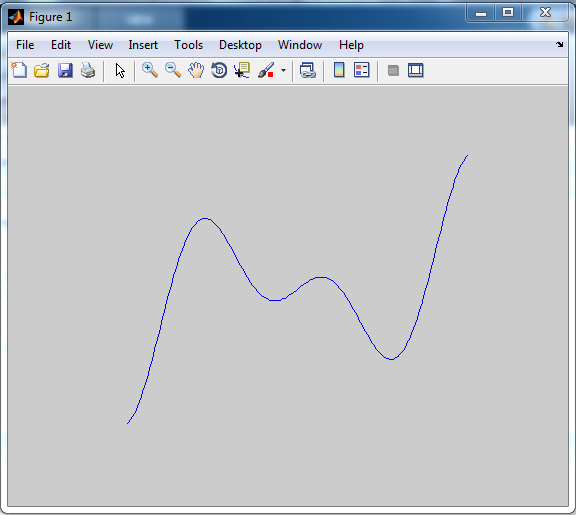
\includegraphics[width=0.5\textwidth]{images/ch4/img_4_5.png}
    \caption{Quitando los axis}
    \label{fig:img_4_5}
\end{figure}

\subsubsection{Escalado de ejes}

Además de permitir una configuración manual de los límites de ejes
mediante la inserción de valores, es posible también establecer límites
mediante modificadores que configuran los ejes y su apariencia de forma
predeterminada. Los más comunes se enlistan y describen en la tabla
siguiente.

\begin{table}[h!]
\centering
\begin{tabular}{ >{\tt}p{3cm} p{5cm} }
\hline
\normalfont\Centering\bfseries Sintaxis  & \Centering\bfseries Descripción \\
\hline 
axis('equal')  & Ajusta el escalado de los ejes de tal modo que sean iguales en cada dirección. \\
axis('square') &  Configura y ajusta la visualización de los ejes a un cuadrado o cubo (3D)  \\
axis('tight') &  Ajusta los ejes al rango de datos disponibles. \\
\hline
\end{tabular}
\caption{Opciones para el escalado de ejes utilizando \texttt{axis}}
\end{table}


\subsection{Añadir texto / anotaciones}

A veces es necesario agregar información extra dentro una gráfica en
forma de texto o anotación. Para ello se puede hacer uso de la función
\texttt{text}, vea el siguiente ejemplo:

\begin{matlab}
t = linspace(0,2*pi);
w = 12;
y = exp(-t).*cos(w*t);
plot(t, y, 'linewidth', 2);
xlabel('Tiempo (s)');
ylabel('Amplitud (mm)');
texto = 'Esto es un texto/anotación';
text(2, 0.5, texto);
\end{matlab}

\begin{figure}[htbp]
    \centering
    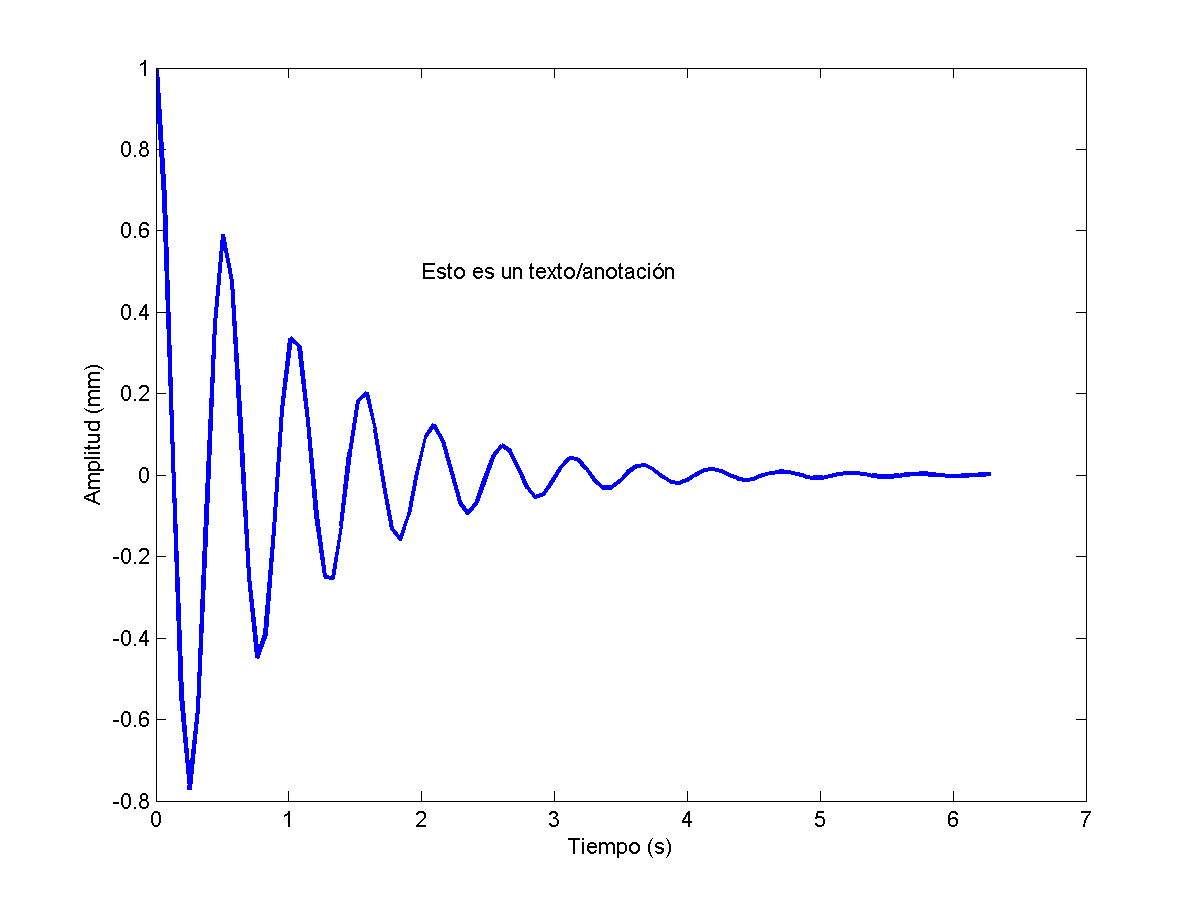
\includegraphics[width=0.75\textwidth]{images/ch4/texto_axes.png}
    \caption{Insertando texto en un axes}
    \label{fig:texto_axes}
\end{figure}

Básicamente la función \texttt{text} necesita tres argumentos de entrada: las 
coordenadas \texttt{x} e \texttt{y} de la posición del texto, y el string 
que contiene el texto que se mostrará en el axes.

\section{Gráficas en coordenadas polares}

En el sistema de coordenadas polares cada punto del plano está definido
por un ángulo y una distancia medidos respecto al eje polar y al polo,
respectivamente. Generalmente para la notación de una ecuación polar se
utilizan la letra griega $\theta$ para el ángulo y una $\rho$ 
para designar la distancia, siendo común la designación $r(\theta)$
para referir a una función en coordenadas polares. \\

Para graficar en coordenadas polares MATLAB dispone de la función polar
cuya sintaxis es:

\begin{matlab}
polar(theta,rho);
\end{matlab}

Ejemplo. Grafique la ecuación $ r(\theta) = \theta $ (espiral).

\begin{matlab}
theta=0:pi/180:6*pi;
r=theta;
polar(theta,r);
\end{matlab}

\begin{figure}[htbp]
    \centering
    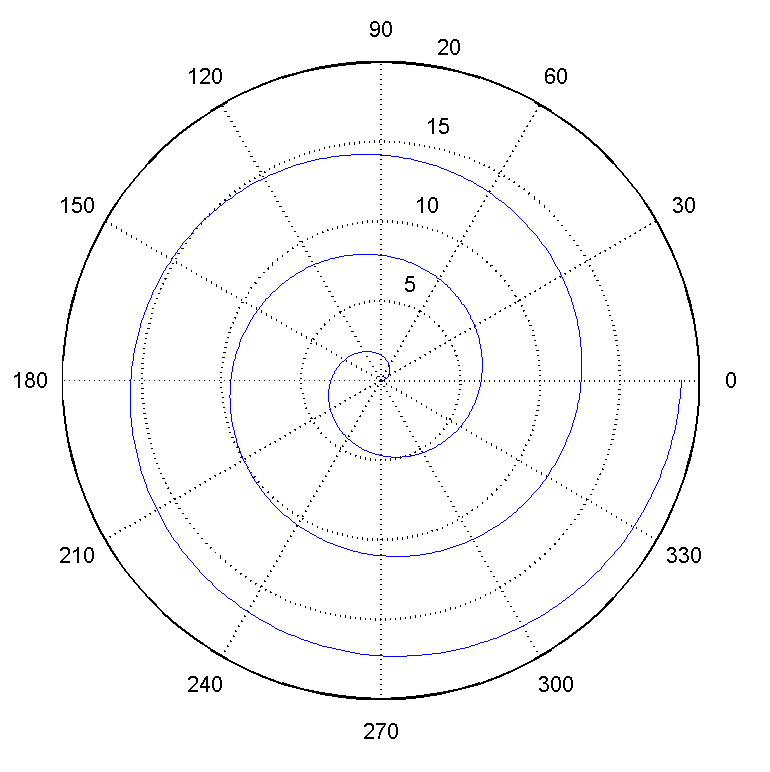
\includegraphics[width=0.6\textwidth]{images/ch4/img_4_6.png}
    \caption{Gráfica de la ecuación $r(\theta) = \theta$}
    \label{fig:img_4_6}
\end{figure}

Pese a que MATLAB cuenta con la función polar para facilitar el trazado
de gráficas en coordenadas polares, es muy sencillo graficar estas
utilizando la función plot con una conversión de coordenadas previa, por
ejemplo, para la misma función anterior:

\begin{matlab}
theta=0:pi/180:6*pi;
r=theta;
x=r.*cos(theta); % Conversión de coordenadas 
y=r.*sin(theta);
plot(x,y);
\end{matlab}

Aunque claro, siempre será mejor utilizar \texttt{polar} dado que esta
automáticamente utiliza los \texttt{axes} de coordenadas polares para
una mejor visualización.


\section{Gráficas de barras}

Las gráficas de barras son una forma de representar gráficamente un conjunto de datos o 
valores y está conformado por barras rectangulares de longitudes proporcionales a los 
valores representados. \\

Para nuestro ejemplo utilizaremos la información proporcionada por la siguiente tabla:

\begin{table}[h!]
\centering
% \rowcolors{1}{}{gray!20}
\begin{tabular}{p{3cm} p{3cm}}
\hline
\Centering\bfseries Asignatura  & \normalfont\bfseries Calificación \\
\hline 
Álgebra & 9 \\
Geometría & 9.5 \\
Cálculo & 10 \\
Estática & 8.5 \\
Química & 8 \\
\hline
\end{tabular}
\caption{Datos para gráfica de barra simple}
\end{table}

MATLAB proporciona la función bar para trazar gráficas de barras, que en su sintaxis más 
simple sólo necesita como argumento un vector con los datos a graficar, véase el ejemplo 
a continuación:

\begin{matlab}
calificaciones=[9,9.5,10,8.5,8];
bar(calificaciones);
\end{matlab}

\begin{figure}[!h]
\centering
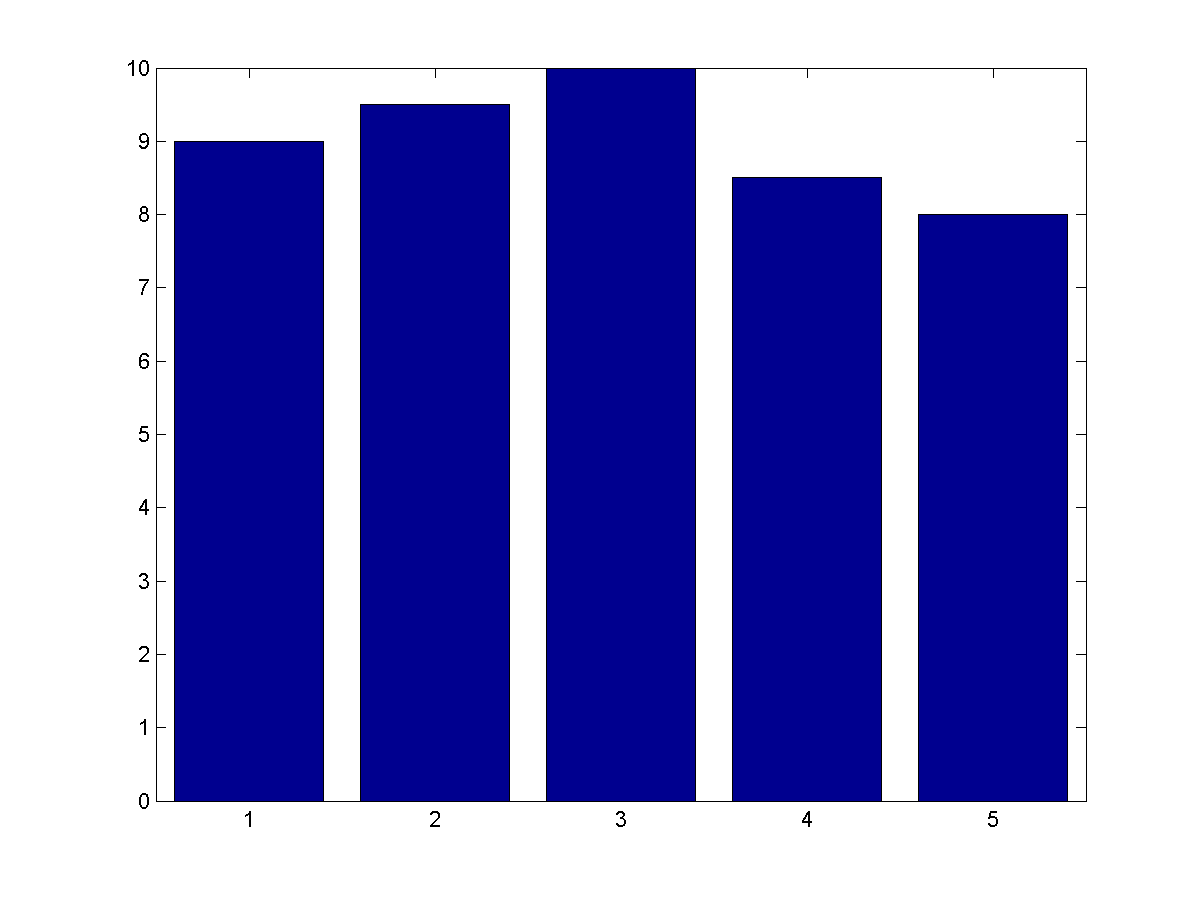
\includegraphics[width=0.6\textwidth]{images/ch4/barra_simple.png}
\caption{Gráficas de barra simple}
\label{fig:barra_simple}
\end{figure}

Lo anterior resulta muy sencillo, pero aún carece de información acerca de los datos que 
se están mostrando. Para añadir una etiqueta a cada dato o barra que se grafica modificaremos 
la propiedad XTickLabel del axes al cuál pertenece el diagrama de barras, en nuestro ejemplo 
esas etiquetas serían el nombre de cada asignatura. Definimos las etiquetas utilizando un 
cell array, veáse el ejemplo:

\begin{matlab}
asignaturas={'Álgebra','Geometría','Cálculo','Estática','Química'};
calificaciones=[9,9.5,10,8.5,8];
h=bar(calificaciones);
set(gca,'XTickLabel',asignaturas);
\end{matlab}

\begin{figure}[!h]
\centering
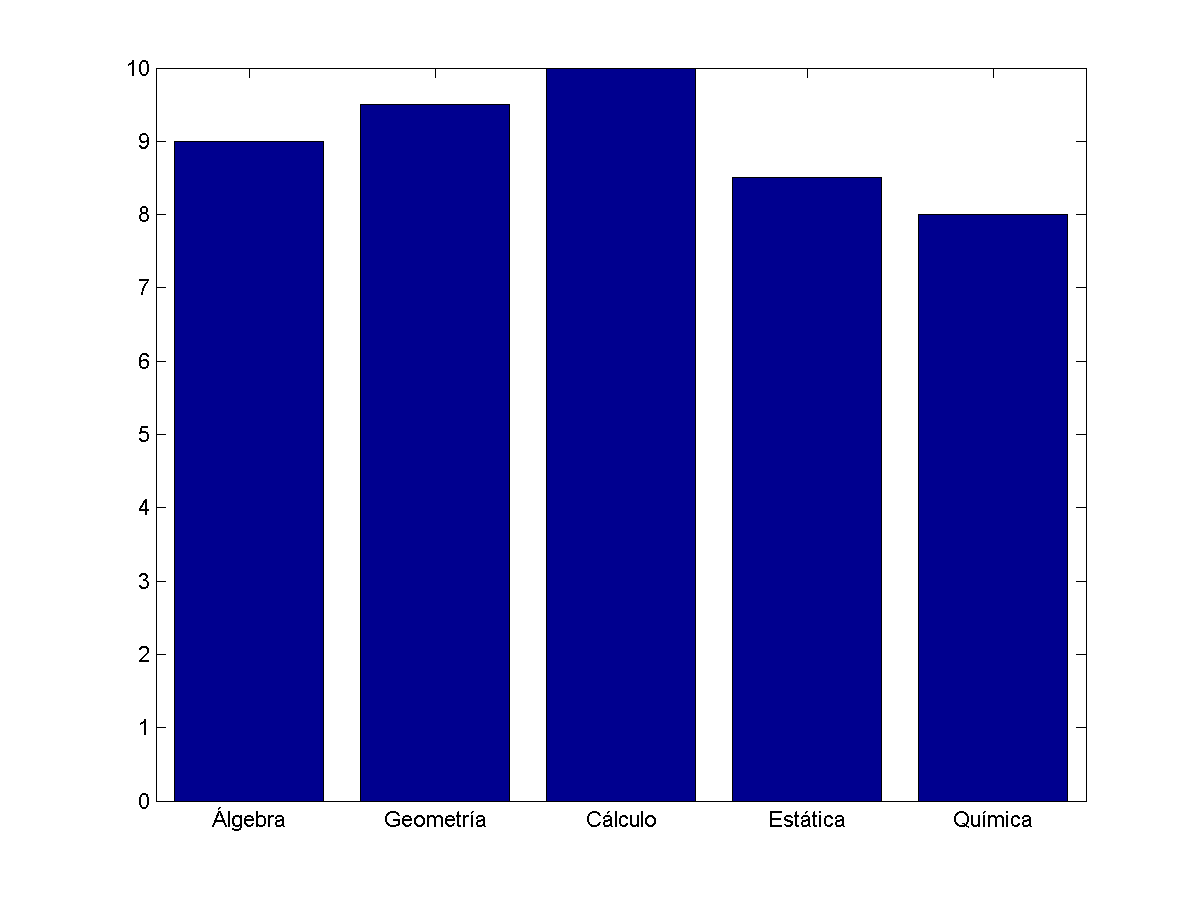
\includegraphics[width=0.6\textwidth]{images/ch4/barra_simple_02.png}
\caption{Gráfica de barra simple, con etiquetas}
\label{fig:barra_simple_02}
\end{figure}

\subsection{Modificar el ancho y color de las barras}

Para modificar el ancho de las barras basta con pasar como segundo argumento de la función bar un 
valor escalar entre 0 y 1, la sintaxis sería:

\begin{verbatim}
bar(X,k);
\end{verbatim}

Donde X es el vector que contiene los valores y k un escalar en el intervalo 0 a 1. \\

Por defecto MATLAB utiliza el color azul para las gráficas de barras, pero existe la posibilidad 
de cambiar el color a conveniencia del usuario. Para ello puede especificarse el color como un 
segundo argumento de la función bar, mediante un especificador de color ('r','g','b','k',...), 
con la sintaxis:

\begin{verbatim}
bar(X,'color');
\end{verbatim}

Donde X es el vector de valor y 'color' el especificador de color mediante caracteres.\\

Si requiere modificar el grosor y color a la vez, puede usar la siguiente sintaxis:

\begin{verbatim}
bar(X,k,'color');
\end{verbatim}

El siguiente ejemplo muestra una gráfica de barras con el ancho y color modificados:

\begin{matlab}
asignaturas={'Álgebra','Geometría','Cálculo','Estática','Química'};
calificaciones=[9,9.5,10,8.5,8];
bar(calificaciones,0.4,'r');
set(gca,'XTickLabel',asignaturas);
title('Calificaciones');
\end{matlab}

\begin{figure}[!h]
\centering
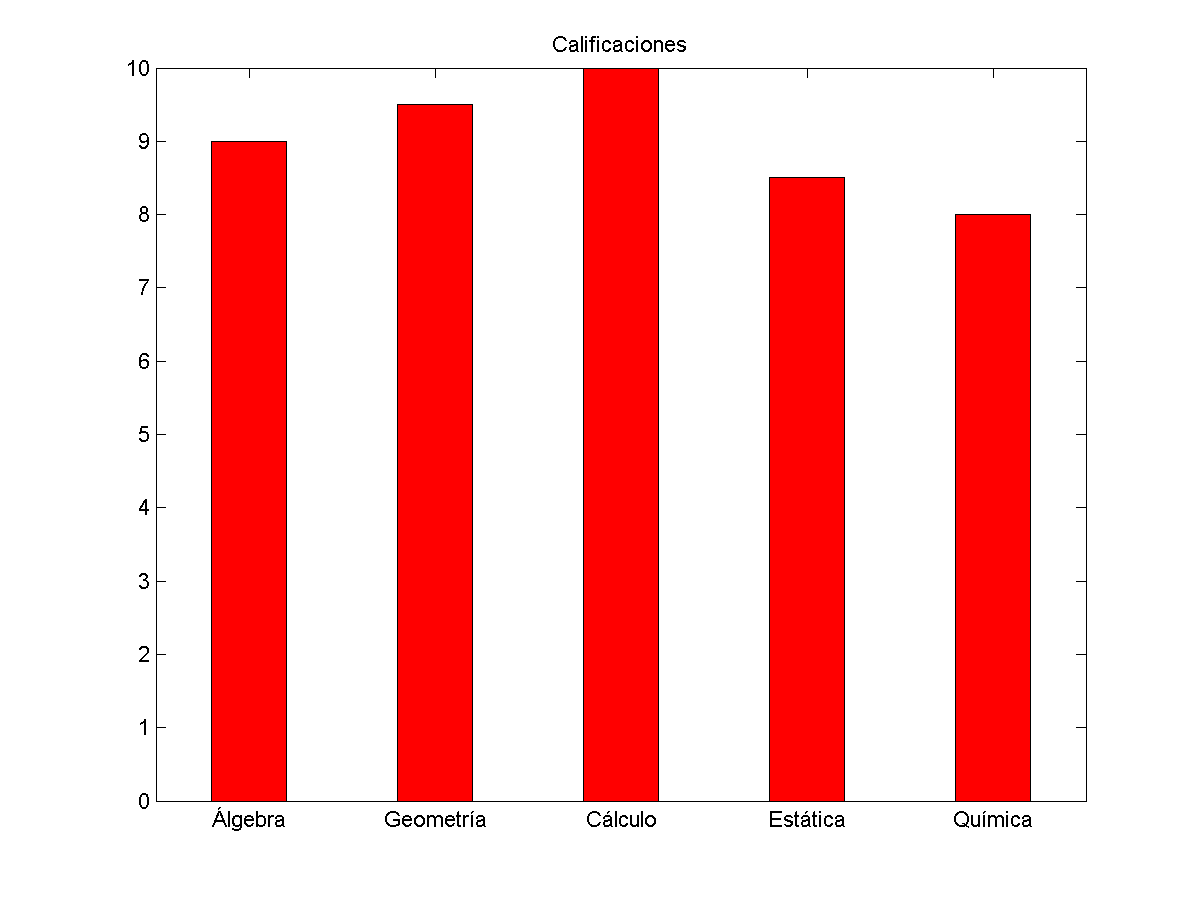
\includegraphics[width=0.6\textwidth]{images/ch4/barra_simple_color.png}
\caption{Gráfica de barra simple, con color y ancho modificado}
\label{fig:barra_simple_color}
\end{figure}

\subsection{Gráficas de barras múltiples}

En ocasiones se necesita representar más de un valor asociado a una misma característica, 
para ello es posible graficar diagramas de barras utilizando matrices en lugar de un vector, 
en donde cada fila proporciona los valores de una misma característica y cada columna pertenece 
a una categoría distinta entre los valores. Para nuestro ejemplo utilizaremos la tabla 
mostrada enseguida.

\begin{table}[h!]
\centering
% \rowcolors{1}{}{gray!20}
\begin{tabular}{p{3cm} P{3cm} P{3cm} P{3cm}}
\hline
\Centering\bfseries \multirow{2}{*}{Alumno} & \normalfont\bfseries \multicolumn{2}{c}{Calificaciones} \\
\cline{2-4}
 & Matemáticas & Física & Química \\
\hline
Ana & 10 & 7 & 9 \\
Jorge & 8 & 8 & 10 \\
Javier & 9 & 9 & 8 \\
\hline
\end{tabular}
\caption{Datos para gráfica de barra simple}
\end{table}

En la tabla anterior cada alumno tiene tres calificaciones asociadas en diferentes asignaturas. 
El siguiente ejemplo muestra cómo trazar la gráfica de barras correspondiente:

\begin{matlab}
nombres={'Ana','Jorge','Javier'};
Ana=[10,7,9];
Jorge=[8,8,10];
Javier=[9,9,8];
bar([Ana;Jorge;Javier]);
set(gca,'XtickLabel',nombres);
\end{matlab}

\begin{figure}[!h]
\centering
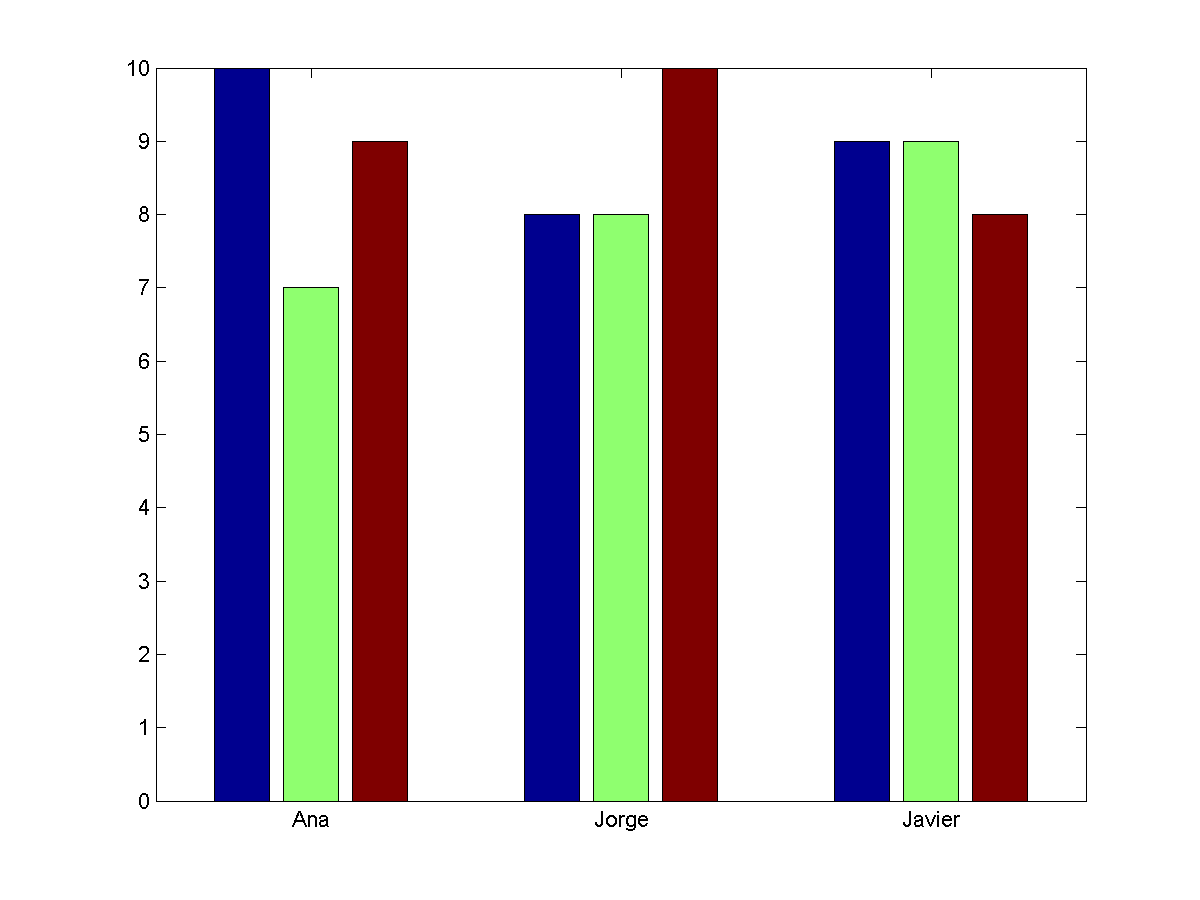
\includegraphics[width=0.6\textwidth]{images/ch4/barra_multiple.png}
\caption{Gráfica de barras múltiples}
\label{fig:barra_multiple}
\end{figure}

\section{Gráficas de pastel/tarta}


\section{Polígonos}



\section{Gráficas de superficies: una primera aproximación}

La representación gráfica de una función de dos variables 
$f(x,y)$ es una superficie trazada en un espacio
tridimensional, resultante de la evaluación de la función en intervalos
determinados para cada variable independiente. \\

A manera de ejemplo crearemos una matriz con los valores resultantes de
la evaluación de la función en un punto específico; comenzaremos
definiendo una función anónima de dos variables y enseguida utilizar
ciclos for anidados para evaluar la función en cada punto. Véase el
ejemplo mostrado a continuación:

\begin{matlab}
f=@(x,y) x.^2+y.^2;
X=-5:0.2:5;
Y=-5:0.2:5;
for i=1:length(X)
    for j=1:length(Y)
        Z(i,j)=f(X(i),Y(j));
    end
end
surf(Z);
\end{matlab}

\begin{figure}[htbp]
    \centering
    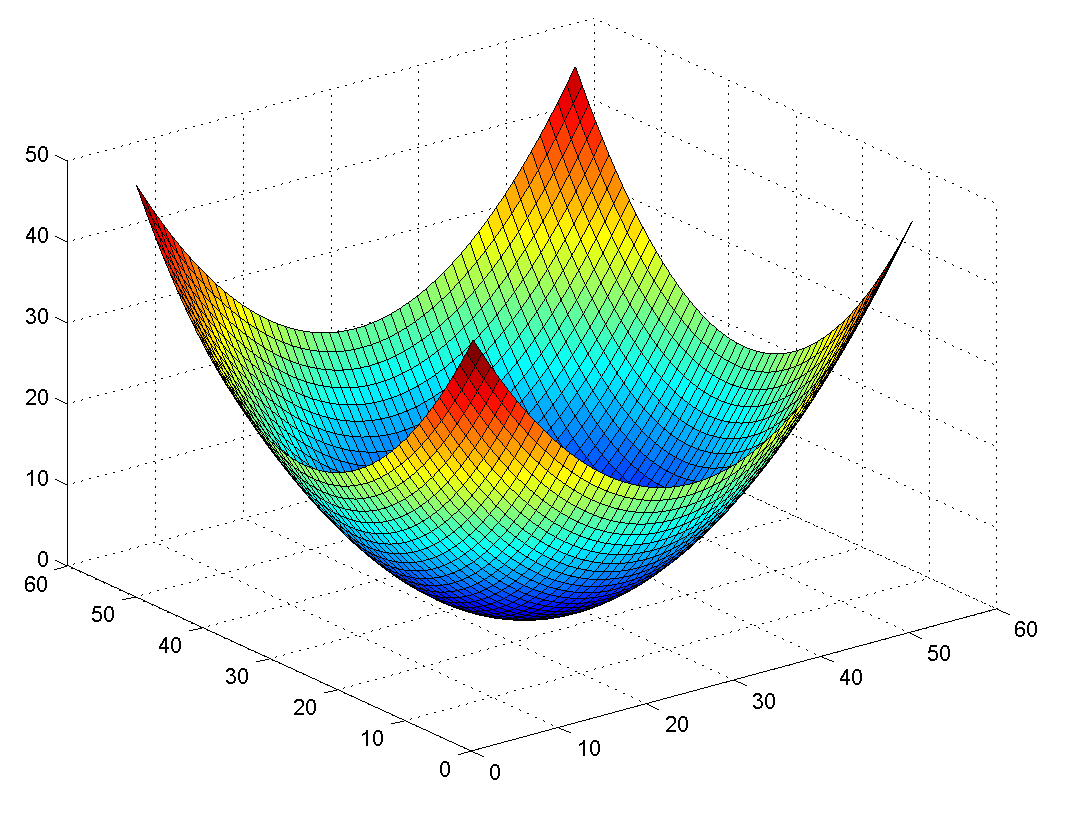
\includegraphics[width=0.6\textwidth]{images/ch4/img_4_7.png}
    \caption{Gráfica de una superficie}
    \label{fig:img_4_7}
\end{figure}

La función \texttt{surf} en el ejemplo anterior recibe como argumento de
entrada una matriz bidimensional cuyos valores corresponden a cada punto
evaluado. El código mostrado es funcional y muy entendible para un
usuario que comienza en el mundo MATLAB, e incluso podría hacerse más
``portable'' o ``reutilizable'' si se definiese como una función, pero
presenta ciertos inconvenientes: los ciclos \texttt{for} en MATLAB son
generalmente conocidos por su lentitud, y más aún, en este caso se
tienen dos ciclos for anidados. Debido a ello, MATLAB proporciona
funciones que realizan la ``tarea'' de evaluar una función de dos
variables en un rango definido mediante la implementación de rejillas
bidimensionales (\texttt{meshgrid}), estas funciones se encuentran
optimizadas mediante la técnica de vectorización y permiten una
ejecución notablemente más veloz.

\section{Gráficas de superficies, utilizando \texttt{meshgrid}}

En el apartado anterior se ha visto como trazar superficies utilizando
ciclos for anidados para crear la matriz que define los valores de la
función de dos variables, pero ahora vamos a optimizar nuestro código
utilizando la función \texttt{meshgrid} para definir el rango de valores
a evaluar, la sintaxis de \texttt{meshgrid} es:

\begin{matlab}
>> [X,Y]=meshgrid(ix,iy);
\end{matlab}

Donde X e Y son las matrices que definen el rango para las variables
independiente y que se utilizarán para evaluar en una determinada
función, ix e iy son vectores que definen el intervalo a evaluar de cada
variable independiente. A continuación se muestra un ejemplo completo de
cómo utilizar meshgrid en conjunto con surf para crear una gráfica de la
función  $f(x,y)=cos(x) sin(y)$:

\begin{matlab}
ix=0:0.2:10;
iy=-5:0.2:5;
[X,Y]=meshgrid(ix,iy);
Z=cos(X).*sin(Y);
surf(X,Y,Z);
\end{matlab}

\begin{figure}[htbp]
    \centering
    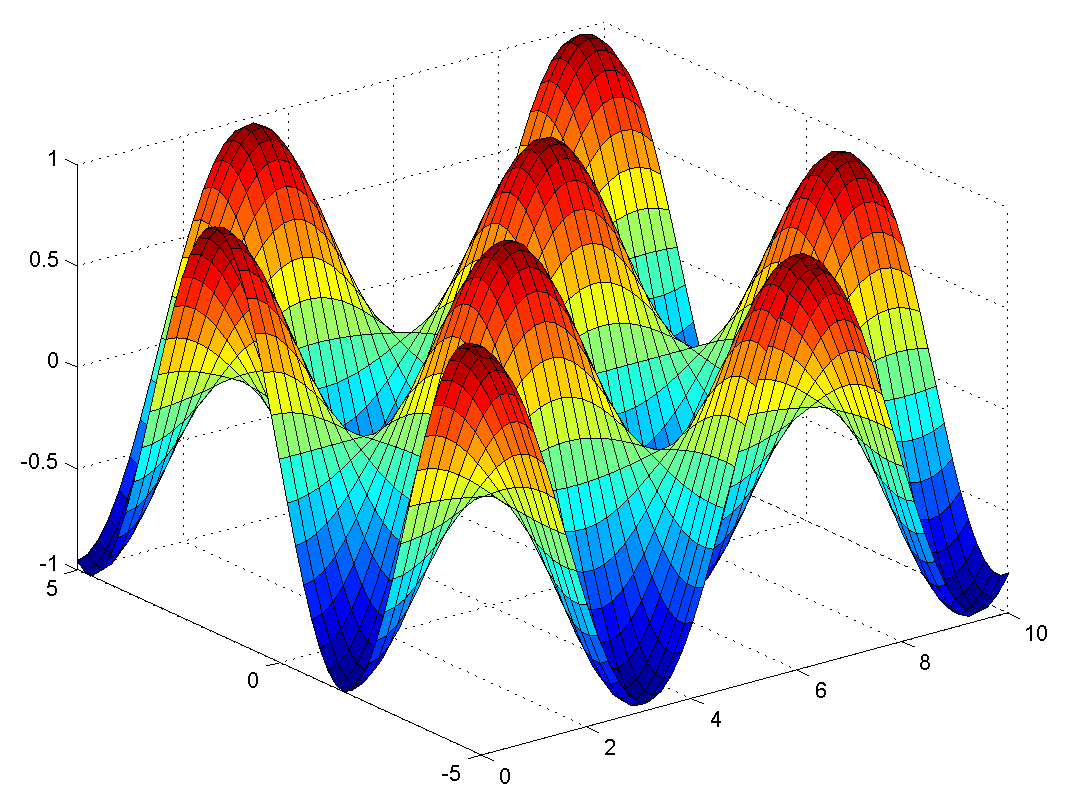
\includegraphics[width=0.6\textwidth]{images/ch4/img_4_8.png}
    \caption{Gráfica de la superficie $f(x)=cos(x) sin(y)$}
    \label{fig:img_4_8}
\end{figure}

Note que las operaciones de multiplicación o división deben estar
vectorizadas, es decir, colocar un punto antes de cada operador
correspondiente para indicar que se debe operar elemento a elemento. De
lo contrario MATLAB devolverá un error o más grave aún: un resultado
incorrecto. \\

Si ambos intervalos X e Y son iguales, puede proporcionar solo un
argumento a la función meshgrid, es decir, es lo mismo tener esto:

\begin{matlab}
[X,Y]=meshgrid(1:10,1:10);
\end{matlab}

que lo siguiente:

\begin{matlab}
[X,Y]=meshgrid(1:10);
\end{matlab}

Claro que por cuestiones de comodidad sería preferible esta última,
aunque quizá afecte un poco la legibilidad de un programa de mayores
dimensiones, pero vamos, nada ``catastrófico''.

\section{Mapas de colores y sombreado}

\subsection{Mapas de colores}

Un mapa de color es, en su definición más simplista, una matriz de m x 3
elementos cuyos valores se encuentran en el intervalo de 0 a 1, y donde
cada fila representa un vector que especifica un color en el formato o
modelo de color RGB. Pero, aquí la cuestión interesante es ¿para qué
sirve un mapa de color?; así pues, un mapa de color no es más que un
conjunto de colores que habrán de utilizarse para ``pintar'' una
superficie de acuerdo a sus valores, pudo notar que en las superficies
trazadas en los apartados anteriores se utiliza un color rojo para los
valores más grandes y un color azul para los más pequeños, pasando por
otras tonalidades para valores intermedios. Debe saber que esa ``forma
de colorear'' la superficie está definida mediante un mapa de color por
defecto, generalmente jet. Aparte de jet MATLAB cuenta con otros mapas
de colores predefinidos que se muestran a continuación:

\begin{figure}[htbp]
\centering
\includegraphics[width=0.25\textwidth]{images/ch4/img_4_9.png}
\caption{}
\end{figure}

Si teclea en MATLAB el nombre de cualquiera de los mapas de colores
mostrados se devuelve una matriz de 64x3 elementos de tipo double, por
ejemplo:

\begin{matlab}
>> map_color=hsv;
>> whos map_color
  Name            Size            Bytes  Class     Attributes

  map_color      64x3              1536  double          
\end{matlab}

Pero todo esto no tiene efecto sobre alguna superficie dibujada, para
cambiar o configurar el mapa de color actual puede utilizar la función
\texttt{colormap}, pasando un mapa de color como argumento, por ejemplo:

\begin{matlab}
[X,Y]=meshgrid(0:0.2:3*pi);
Z=cos(X).*sin(Y);
surf(X,Y,Z);
colormap(hot);
\end{matlab}

\begin{figure}[htbp]
    \centering
    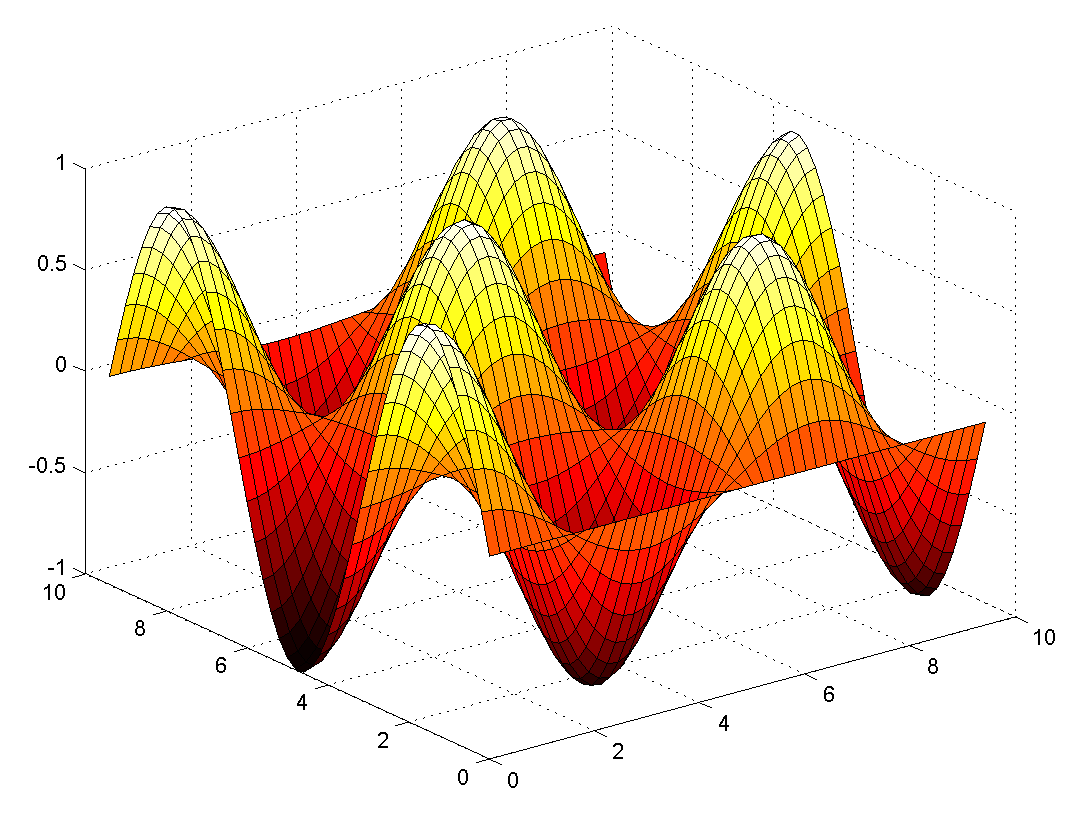
\includegraphics[width=0.6\textwidth]{images/ch4/img_4_10.png}
    \caption{Utilizando el mapa de color \texttt{hot}}
    \label{fig:label}
\end{figure}

Interesante, sobre todo para quienes deseen darle a sus gráficos una
mayor calidad estética o acorde a los datos que esté representando. \\

Si por alguna razón ninguno de los mapas de colores predefinidos le
``convence'', puede definir su propio mapa de color sin muchas
complicaciones, para ello debe crear una matriz de m x 3 elementos donde
cada fila contenga información acerca de un color en formato RGB,
tomando en cuenta que el color ubicado en la primera fila será asignado
al valor más pequeño y la última fila al mayor. Revise el siguiente
ejemplo en el cual se define un mapa de color mediante cierta secuencia:

\begin{matlab}
Z=membrane;
surf(Z);
v=(1:10)'/10;
cmap=[v flipud(v) flipud(v)];
colormap(cmap);
\end{matlab}

\begin{figure}[htbp]
    \centering
    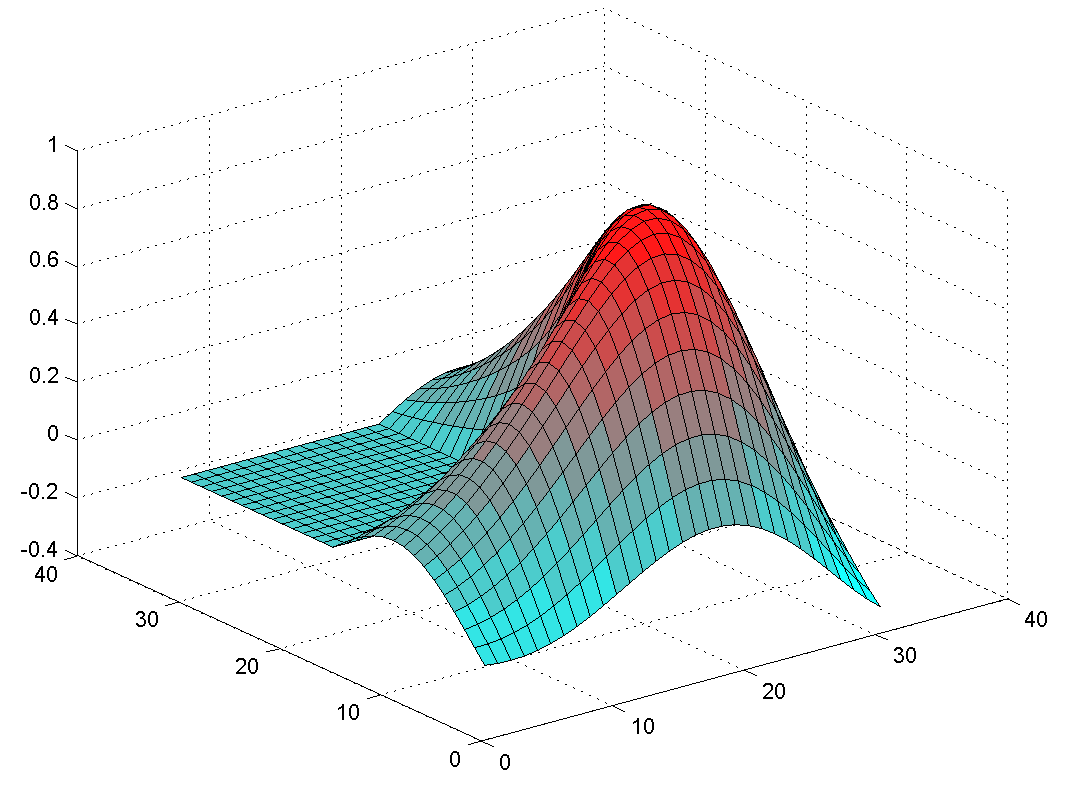
\includegraphics[width=0.75\textwidth]{images/ch4/img_4_11.png}
    \caption{Utilizando un mapa de color personalizado}
    \label{fig:img_4_11}
\end{figure}

El resultado es una interesante variación de tonalidades ¿azul? a rojo.
Por supuesto que usted tiene todas las libertades para experimentar con
diversas secuencias de colores y ``adoptar'' la que mejor le resulte.

\subsection{Sombreado}

Para efectos de esta sección, con sombreado se refiere a la forma en que
MATLAB \emph{pinta} o \emph{rellena} los diversos componentes o parches
(patch) que conforman una superficie. \\

En MATLAB existen tres tipos de sombreado que pueden controlarse
mediante la función \texttt{shading}, los cuales son:

\begin{itemize}
\tightlist
\item
  faceted
\item
  flat
\item
  interp
\end{itemize}

El tipo \texttt{faceted} es el sombreado por defecto, y se caracteriza
por pintar cada parche de la superficie utilizando un color sólido de
relleno y un borde en color negro. \\

El tipo \texttt{flat} funciona de manera similar al anterior, con la
diferencia que el borde adquiere el mismo color que el interior del
parche. \\

Y el tipo \texttt{interp} se vale de una interpolación de la matriz que
define el mapa de color actual para pintar de forma cuasi-continua y con
variaciones menos ``bruscas'' a cada parche, de hecho con este tipo de
sombreado es imposible distinguir cada pieza que compone la superficie. \\

La función \texttt{shading} sólo necesita como argumento el tipo de
sombreado, por ejemplo:

\begin{matlab}
>> shading('flat')
\end{matlab}

Incluso acepta la notación de comandos, es decir, la siguiente forma
también es válida:

\begin{matlab}
>> shading flat
\end{matlab}

\section{Planos}

\section{Esferas}

\section{Cilindros}

\section{Curvas de nivel}

\section{Subplots: múltiples axes}

\section{Gráficos interactivos}